\documentclass[1p]{elsarticle_modified}
%\bibliographystyle{elsarticle-num}

%\usepackage[colorlinks]{hyperref}
%\usepackage{abbrmath_seonhwa} %\Abb, \Ascr, \Acal ,\Abf, \Afrak
\usepackage{amsfonts}
\usepackage{amssymb}
\usepackage{amsmath}
\usepackage{amsthm}
\usepackage{scalefnt}
\usepackage{amsbsy}
\usepackage{kotex}
\usepackage{caption}
\usepackage{subfig}
\usepackage{color}
\usepackage{graphicx}
\usepackage{xcolor} %% white, black, red, green, blue, cyan, magenta, yellow
\usepackage{float}
\usepackage{setspace}
\usepackage{hyperref}

\usepackage{tikz}
\usetikzlibrary{arrows}

\usepackage{multirow}
\usepackage{array} % fixed length table
\usepackage{hhline}

%%%%%%%%%%%%%%%%%%%%%
\makeatletter
\renewcommand*\env@matrix[1][\arraystretch]{%
	\edef\arraystretch{#1}%
	\hskip -\arraycolsep
	\let\@ifnextchar\new@ifnextchar
	\array{*\c@MaxMatrixCols c}}
\makeatother %https://tex.stackexchange.com/questions/14071/how-can-i-increase-the-line-spacing-in-a-matrix
%%%%%%%%%%%%%%%

\usepackage[normalem]{ulem}

\newcommand{\msout}[1]{\ifmmode\text{\sout{\ensuremath{#1}}}\else\sout{#1}\fi}
%SOURCE: \msout is \stkout macro in https://tex.stackexchange.com/questions/20609/strikeout-in-math-mode

\newcommand{\cancel}[1]{
	\ifmmode
	{\color{red}\msout{#1}}
	\else
	{\color{red}\sout{#1}}
	\fi
}

\newcommand{\add}[1]{
	{\color{blue}\uwave{#1}}
}

\newcommand{\replace}[2]{
	\ifmmode
	{\color{red}\msout{#1}}{\color{blue}\uwave{#2}}
	\else
	{\color{red}\sout{#1}}{\color{blue}\uwave{#2}}
	\fi
}

\newcommand{\Sol}{\mathcal{S}} %segment
\newcommand{\D}{D} %diagram
\newcommand{\A}{\mathcal{A}} %arc


%%%%%%%%%%%%%%%%%%%%%%%%%%%%%5 test

\def\sl{\operatorname{\textup{SL}}(2,\Cbb)}
\def\psl{\operatorname{\textup{PSL}}(2,\Cbb)}
\def\quan{\mkern 1mu \triangleright \mkern 1mu}

\theoremstyle{definition}
\newtheorem{thm}{Theorem}[section]
\newtheorem{prop}[thm]{Proposition}
\newtheorem{lem}[thm]{Lemma}
\newtheorem{ques}[thm]{Question}
\newtheorem{cor}[thm]{Corollary}
\newtheorem{defn}[thm]{Definition}
\newtheorem{exam}[thm]{Example}
\newtheorem{rmk}[thm]{Remark}
\newtheorem{alg}[thm]{Algorithm}

\newcommand{\I}{\sqrt{-1}}
\begin{document}

%\begin{frontmatter}
%
%\title{Boundary parabolic representations of knots up to 8 crossings}
%
%%% Group authors per affiliation:
%\author{Yunhi Cho} 
%\address{Department of Mathematics, University of Seoul, Seoul, Korea}
%\ead{yhcho@uos.ac.kr}
%
%
%\author{Seonhwa Kim} %\fnref{s_kim}}
%\address{Center for Geometry and Physics, Institute for Basic Science, Pohang, 37673, Korea}
%\ead{ryeona17@ibs.re.kr}
%
%\author{Hyuk Kim}
%\address{Department of Mathematical Sciences, Seoul National University, Seoul 08826, Korea}
%\ead{hyukkim@snu.ac.kr}
%
%\author{Seokbeom Yoon}
%\address{Department of Mathematical Sciences, Seoul National University, Seoul, 08826,  Korea}
%\ead{sbyoon15@snu.ac.kr}
%
%\begin{abstract}
%We find all boundary parabolic representation of knots up to 8 crossings.
%
%\end{abstract}
%\begin{keyword}
%    \MSC[2010] 57M25 
%\end{keyword}
%
%\end{frontmatter}

%\linenumbers
%\tableofcontents
%
\newcommand\colored[1]{\textcolor{white}{\rule[-0.35ex]{0.8em}{1.4ex}}\kern-0.8em\color{red} #1}%
%\newcommand\colored[1]{\textcolor{white}{ #1}\kern-2.17ex	\textcolor{white}{ #1}\kern-1.81ex	\textcolor{white}{ #1}\kern-2.15ex\color{red}#1	}

{\Large $\underline{12a_{0601}~(K12a_{0601})}$}

\setlength{\tabcolsep}{10pt}
\renewcommand{\arraystretch}{1.6}
\vspace{1cm}\begin{tabular}{m{100pt}>{\centering\arraybackslash}m{274pt}}
\multirow{5}{120pt}{
	\centering
	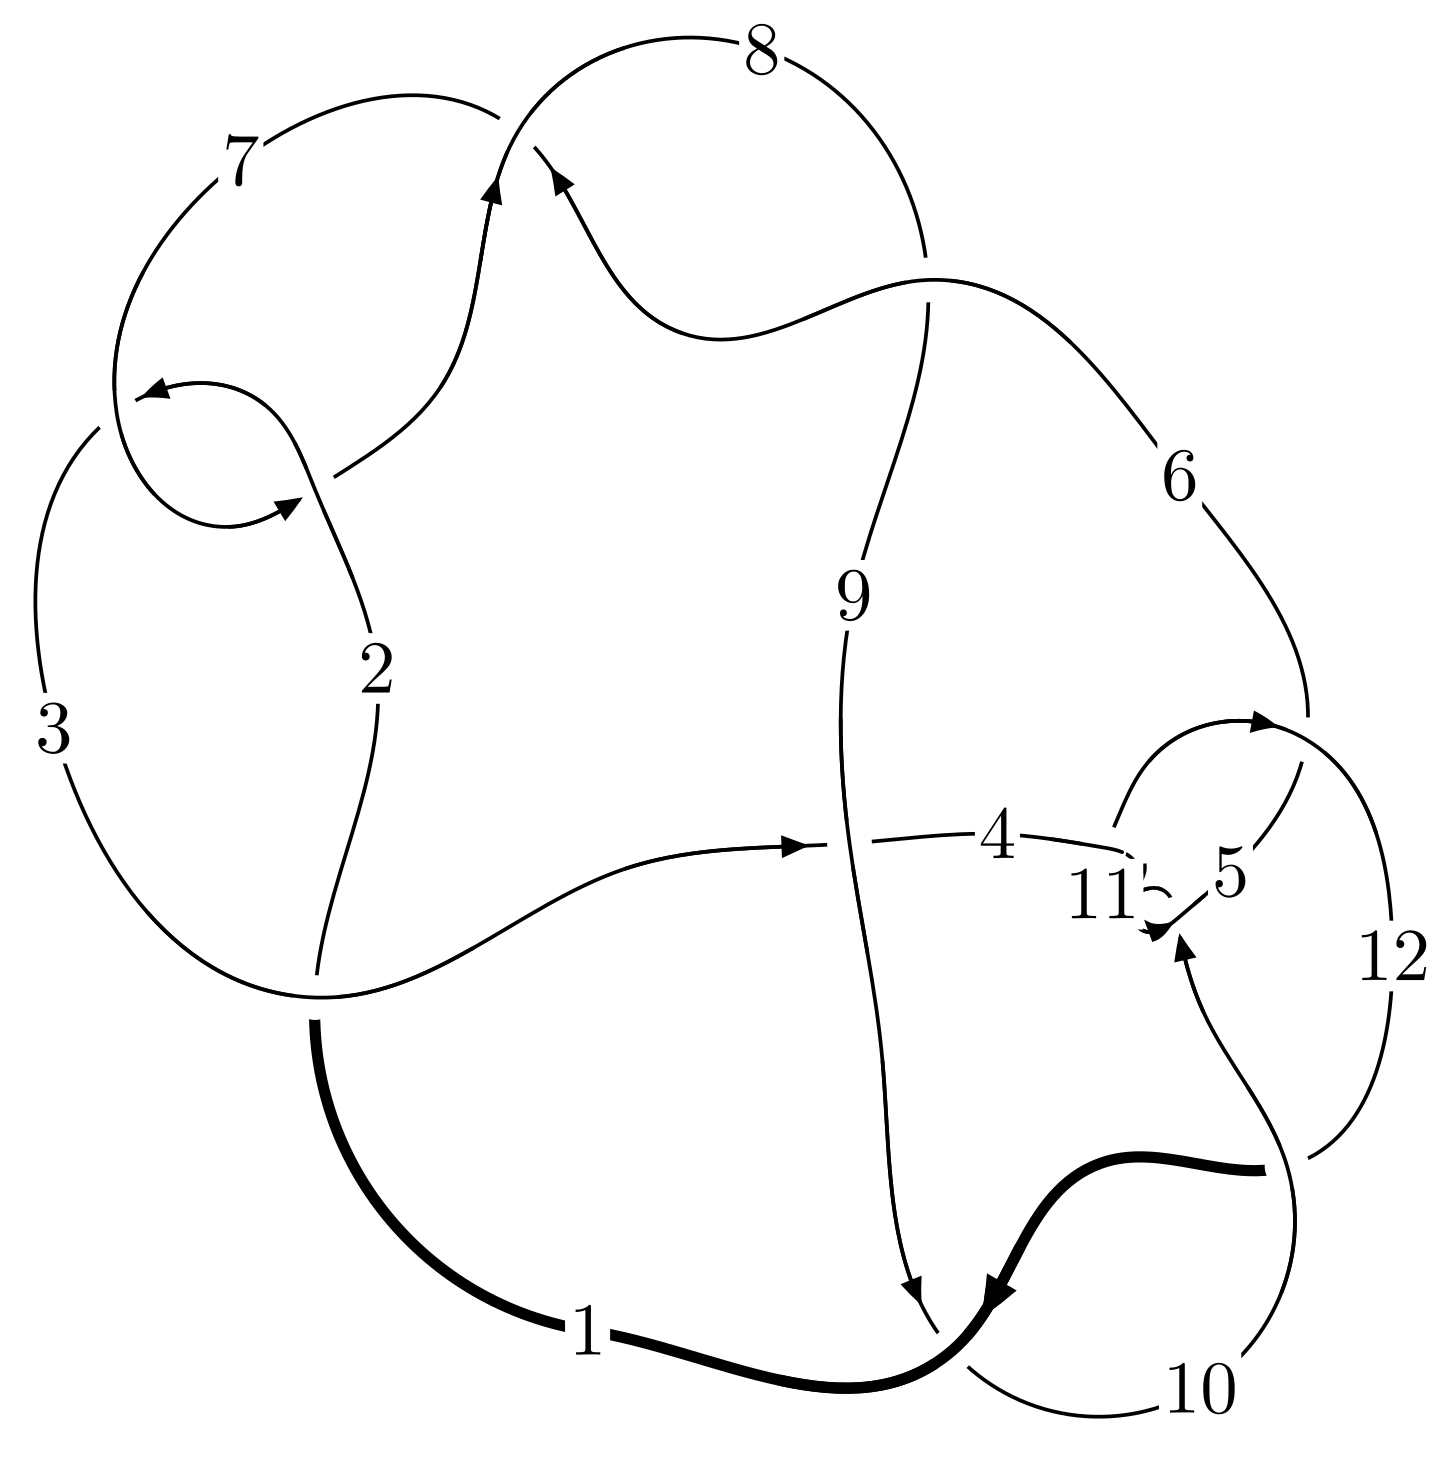
\includegraphics[width=112pt]{../../../GIT/diagram.site/Diagrams/png/1402_12a_0601.png}\\
\ \ \ A knot diagram\footnotemark}&
\allowdisplaybreaks
\textbf{Linearized knot diagam} \\
\cline{2-2}
 &
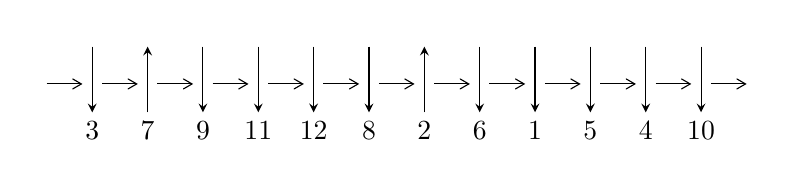
\begin{tikzpicture}[x=20pt, y=17pt]
	% nodes
	\node (C0) at (0, 0) {};
	\node (C1) at (1, 0) {};
	\node (C1U) at (1, +1) {};
	\node (C1D) at (1, -1) {3};

	\node (C2) at (2, 0) {};
	\node (C2U) at (2, +1) {};
	\node (C2D) at (2, -1) {7};

	\node (C3) at (3, 0) {};
	\node (C3U) at (3, +1) {};
	\node (C3D) at (3, -1) {9};

	\node (C4) at (4, 0) {};
	\node (C4U) at (4, +1) {};
	\node (C4D) at (4, -1) {11};

	\node (C5) at (5, 0) {};
	\node (C5U) at (5, +1) {};
	\node (C5D) at (5, -1) {12};

	\node (C6) at (6, 0) {};
	\node (C6U) at (6, +1) {};
	\node (C6D) at (6, -1) {8};

	\node (C7) at (7, 0) {};
	\node (C7U) at (7, +1) {};
	\node (C7D) at (7, -1) {2};

	\node (C8) at (8, 0) {};
	\node (C8U) at (8, +1) {};
	\node (C8D) at (8, -1) {6};

	\node (C9) at (9, 0) {};
	\node (C9U) at (9, +1) {};
	\node (C9D) at (9, -1) {1};

	\node (C10) at (10, 0) {};
	\node (C10U) at (10, +1) {};
	\node (C10D) at (10, -1) {5};

	\node (C11) at (11, 0) {};
	\node (C11U) at (11, +1) {};
	\node (C11D) at (11, -1) {4};

	\node (C12) at (12, 0) {};
	\node (C12U) at (12, +1) {};
	\node (C12D) at (12, -1) {10};
	\node (C13) at (13, 0) {};

	% arrows
	\draw[->,>={angle 60}]
	(C0) edge (C1) (C1) edge (C2) (C2) edge (C3) (C3) edge (C4) (C4) edge (C5) (C5) edge (C6) (C6) edge (C7) (C7) edge (C8) (C8) edge (C9) (C9) edge (C10) (C10) edge (C11) (C11) edge (C12) (C12) edge (C13) ;	\draw[->,>=stealth]
	(C1U) edge (C1D) (C2D) edge (C2U) (C3U) edge (C3D) (C4U) edge (C4D) (C5U) edge (C5D) (C6U) edge (C6D) (C7D) edge (C7U) (C8U) edge (C8D) (C9U) edge (C9D) (C10U) edge (C10D) (C11U) edge (C11D) (C12U) edge (C12D) ;
	\end{tikzpicture} \\
\hhline{~~} \\& 
\textbf{Solving Sequence} \\ \cline{2-2} 
 &
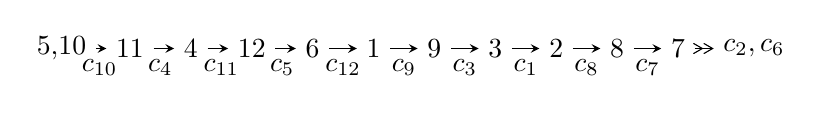
\begin{tikzpicture}[x=22pt, y=7pt]
	% node
	\node (A0) at (-1/8, 0) {5,10};
	\node (A1) at (1, 0) {11};
	\node (A2) at (2, 0) {4};
	\node (A3) at (3, 0) {12};
	\node (A4) at (4, 0) {6};
	\node (A5) at (5, 0) {1};
	\node (A6) at (6, 0) {9};
	\node (A7) at (7, 0) {3};
	\node (A8) at (8, 0) {2};
	\node (A9) at (9, 0) {8};
	\node (A10) at (10, 0) {7};
	\node (C1) at (1/2, -1) {$c_{10}$};
	\node (C2) at (3/2, -1) {$c_{4}$};
	\node (C3) at (5/2, -1) {$c_{11}$};
	\node (C4) at (7/2, -1) {$c_{5}$};
	\node (C5) at (9/2, -1) {$c_{12}$};
	\node (C6) at (11/2, -1) {$c_{9}$};
	\node (C7) at (13/2, -1) {$c_{3}$};
	\node (C8) at (15/2, -1) {$c_{1}$};
	\node (C9) at (17/2, -1) {$c_{8}$};
	\node (C10) at (19/2, -1) {$c_{7}$};
	\node (A11) at (45/4, 0) {$c_{2},c_{6}$};

	% edge
	\draw[->,>=stealth]	
	(A0) edge (A1) (A1) edge (A2) (A2) edge (A3) (A3) edge (A4) (A4) edge (A5) (A5) edge (A6) (A6) edge (A7) (A7) edge (A8) (A8) edge (A9) (A9) edge (A10) ;
	\draw[->>,>={angle 60}]	
	(A10) edge (A11);
\end{tikzpicture} \\ 

\end{tabular} \\

\footnotetext{
The image of knot diagram is generated by the software ``\textbf{Draw programme}" developed by Andrew Bartholomew(\url{http://www.layer8.co.uk/maths/draw/index.htm\#Running-draw}), where we modified some parts for our purpose(\url{https://github.com/CATsTAILs/LinksPainter}).
}\phantom \\ \newline 
\centering \textbf{Ideals for irreducible components\footnotemark of $X_{\text{par}}$} 
 
\begin{align*}
I^u_{1}&=\langle 
u^{63}+u^{62}+\cdots+4 u+1\rangle \\
\\
\end{align*}
\raggedright * 1 irreducible components of $\dim_{\mathbb{C}}=0$, with total 63 representations.\\
\footnotetext{All coefficients of polynomials are rational numbers. But the coefficients are sometimes approximated in decimal forms when there is not enough margin.}
\newpage
\renewcommand{\arraystretch}{1}
\centering \section*{I. $I^u_{1}= \langle u^{63}+u^{62}+\cdots+4 u+1 \rangle$}
\flushleft \textbf{(i) Arc colorings}\\
\begin{tabular}{m{7pt} m{180pt} m{7pt} m{180pt} }
\flushright $a_{5}=$&$\begin{pmatrix}0\\u\end{pmatrix}$ \\
\flushright $a_{10}=$&$\begin{pmatrix}1\\0\end{pmatrix}$ \\
\flushright $a_{11}=$&$\begin{pmatrix}1\\u^2\end{pmatrix}$ \\
\flushright $a_{4}=$&$\begin{pmatrix}u\\u^3+u\end{pmatrix}$ \\
\flushright $a_{12}=$&$\begin{pmatrix}u^2+1\\u^4+2 u^2\end{pmatrix}$ \\
\flushright $a_{6}=$&$\begin{pmatrix}- u^5-2 u^3- u\\- u^7-3 u^5-2 u^3+u\end{pmatrix}$ \\
\flushright $a_{1}=$&$\begin{pmatrix}- u^4- u^2+1\\u^4+2 u^2\end{pmatrix}$ \\
\flushright $a_{9}=$&$\begin{pmatrix}u^8+3 u^6+u^4-2 u^2+1\\- u^8-4 u^6-4 u^4\end{pmatrix}$ \\
\flushright $a_{3}=$&$\begin{pmatrix}u^{19}+8 u^{17}+24 u^{15}+30 u^{13}+7 u^{11}-10 u^9+4 u^7+6 u^5-3 u^3+2 u\\- u^{19}-9 u^{17}-32 u^{15}-55 u^{13}-43 u^{11}-9 u^9-4 u^5+u^3+u\end{pmatrix}$ \\
\flushright $a_{2}=$&$\begin{pmatrix}- u^{34}-15 u^{32}+\cdots+u^2+1\\u^{34}+16 u^{32}+\cdots-2 u^4+3 u^2\end{pmatrix}$ \\
\flushright $a_{8}=$&$\begin{pmatrix}- u^{20}-9 u^{18}+\cdots- u^2+1\\- u^{22}-10 u^{20}+\cdots+2 u^4- u^2\end{pmatrix}$ \\
\flushright $a_{7}=$&$\begin{pmatrix}- u^{35}-16 u^{33}+\cdots+3 u^3-2 u\\- u^{37}-17 u^{35}+\cdots- u^3+u\end{pmatrix}$\\&\end{tabular}
\flushleft \textbf{(ii) Obstruction class $= -1$}\\~\\
\flushleft \textbf{(iii) Cusp Shapes $= -4 u^{62}-4 u^{61}+\cdots-40 u-18$}\\~\\
\newpage\renewcommand{\arraystretch}{1}
\flushleft \textbf{(iv) u-Polynomials at the component}\newline \\
\begin{tabular}{m{50pt}|m{274pt}}
Crossings & \hspace{64pt}u-Polynomials at each crossing \\
\hline $$\begin{aligned}c_{1},c_{6},c_{8}\end{aligned}$$&$\begin{aligned}
&u^{63}+15 u^{62}+\cdots+16 u^2-1
\end{aligned}$\\
\hline $$\begin{aligned}c_{2},c_{7}\end{aligned}$$&$\begin{aligned}
&u^{63}+u^{62}+\cdots+2 u^3+1
\end{aligned}$\\
\hline $$\begin{aligned}c_{3}\end{aligned}$$&$\begin{aligned}
&u^{63}+u^{62}+\cdots+11678 u+2941
\end{aligned}$\\
\hline $$\begin{aligned}c_{4},c_{10},c_{11}\end{aligned}$$&$\begin{aligned}
&u^{63}+u^{62}+\cdots+4 u+1
\end{aligned}$\\
\hline $$\begin{aligned}c_{5}\end{aligned}$$&$\begin{aligned}
&u^{63}- u^{62}+\cdots+394 u+65
\end{aligned}$\\
\hline $$\begin{aligned}c_{9},c_{12}\end{aligned}$$&$\begin{aligned}
&u^{63}-9 u^{62}+\cdots+16 u+1
\end{aligned}$\\
\hline
\end{tabular}\\~\\
\newpage\renewcommand{\arraystretch}{1}
\flushleft \textbf{(v) Riley Polynomials at the component}\newline \\
\begin{tabular}{m{50pt}|m{274pt}}
Crossings & \hspace{64pt}Riley Polynomials at each crossing \\
\hline $$\begin{aligned}c_{1},c_{6},c_{8}\end{aligned}$$&$\begin{aligned}
&y^{63}+67 y^{62}+\cdots+32 y-1
\end{aligned}$\\
\hline $$\begin{aligned}c_{2},c_{7}\end{aligned}$$&$\begin{aligned}
&y^{63}+15 y^{62}+\cdots+16 y^2-1
\end{aligned}$\\
\hline $$\begin{aligned}c_{3}\end{aligned}$$&$\begin{aligned}
&y^{63}+27 y^{62}+\cdots-133314016 y-8649481
\end{aligned}$\\
\hline $$\begin{aligned}c_{4},c_{10},c_{11}\end{aligned}$$&$\begin{aligned}
&y^{63}+59 y^{62}+\cdots-16 y^2-1
\end{aligned}$\\
\hline $$\begin{aligned}c_{5}\end{aligned}$$&$\begin{aligned}
&y^{63}+23 y^{62}+\cdots-226184 y-4225
\end{aligned}$\\
\hline $$\begin{aligned}c_{9},c_{12}\end{aligned}$$&$\begin{aligned}
&y^{63}+55 y^{62}+\cdots+208 y-1
\end{aligned}$\\
\hline
\end{tabular}\\~\\
\newpage\flushleft \textbf{(vi) Complex Volumes and Cusp Shapes}
$$\begin{array}{c|c|c}  
\text{Solutions to }I^u_{1}& \I (\text{vol} + \sqrt{-1}CS) & \text{Cusp shape}\\
 \hline 
\begin{aligned}
u &= \phantom{-}0.026966 + 1.106350 I\end{aligned}
 & \phantom{-}5.72389 + 2.98502 I & \phantom{-0.000000 } 0 \\ \hline\begin{aligned}
u &= \phantom{-}0.026966 - 1.106350 I\end{aligned}
 & \phantom{-}5.72389 - 2.98502 I & \phantom{-0.000000 } 0 \\ \hline\begin{aligned}
u &= -0.687201 + 0.412506 I\end{aligned}
 & \phantom{-}9.24727 + 10.49800 I & -3.51356 - 8.27768 I \\ \hline\begin{aligned}
u &= -0.687201 - 0.412506 I\end{aligned}
 & \phantom{-}9.24727 - 10.49800 I & -3.51356 + 8.27768 I \\ \hline\begin{aligned}
u &= \phantom{-}0.683558 + 0.418042 I\end{aligned}
 & \phantom{-}9.63540 - 4.12275 I & -2.71858 + 3.42597 I \\ \hline\begin{aligned}
u &= \phantom{-}0.683558 - 0.418042 I\end{aligned}
 & \phantom{-}9.63540 + 4.12275 I & -2.71858 - 3.42597 I \\ \hline\begin{aligned}
u &= \phantom{-}0.594200 + 0.519837 I\end{aligned}
 & \phantom{-}10.03370 - 0.13330 I & -1.68361 + 2.69330 I \\ \hline\begin{aligned}
u &= \phantom{-}0.594200 - 0.519837 I\end{aligned}
 & \phantom{-}10.03370 + 0.13330 I & -1.68361 - 2.69330 I \\ \hline\begin{aligned}
u &= -0.587406 + 0.526285 I\end{aligned}
 & \phantom{-}9.69166 - 6.24596 I & -2.31699 + 2.22181 I \\ \hline\begin{aligned}
u &= -0.587406 - 0.526285 I\end{aligned}
 & \phantom{-}9.69166 + 6.24596 I & -2.31699 - 2.22181 I \\ \hline\begin{aligned}
u &= \phantom{-}0.132381 + 1.218840 I\end{aligned}
 & \phantom{-}0.146145 - 0.270553 I & \phantom{-0.000000 } 0 \\ \hline\begin{aligned}
u &= \phantom{-}0.132381 - 1.218840 I\end{aligned}
 & \phantom{-}0.146145 + 0.270553 I & \phantom{-0.000000 } 0 \\ \hline\begin{aligned}
u &= -0.657132 + 0.390763 I\end{aligned}
 & \phantom{-}1.28852 + 6.79003 I & -7.72888 - 9.43258 I \\ \hline\begin{aligned}
u &= -0.657132 - 0.390763 I\end{aligned}
 & \phantom{-}1.28852 - 6.79003 I & -7.72888 + 9.43258 I \\ \hline\begin{aligned}
u &= \phantom{-}0.636380 + 0.414397 I\end{aligned}
 & \phantom{-}3.22883 - 2.96613 I & -2.26029 + 3.71050 I \\ \hline\begin{aligned}
u &= \phantom{-}0.636380 - 0.414397 I\end{aligned}
 & \phantom{-}3.22883 + 2.96613 I & -2.26029 - 3.71050 I \\ \hline\begin{aligned}
u &= \phantom{-}0.588036 + 0.455040 I\end{aligned}
 & \phantom{-}3.42044 - 1.03125 I & -1.58884 + 3.34604 I \\ \hline\begin{aligned}
u &= \phantom{-}0.588036 - 0.455040 I\end{aligned}
 & \phantom{-}3.42044 + 1.03125 I & -1.58884 - 3.34604 I \\ \hline\begin{aligned}
u &= -0.546794 + 0.481840 I\end{aligned}
 & \phantom{-}1.71497 - 2.81621 I & -6.17352 + 3.05233 I \\ \hline\begin{aligned}
u &= -0.546794 - 0.481840 I\end{aligned}
 & \phantom{-}1.71497 + 2.81621 I & -6.17352 - 3.05233 I \\ \hline\begin{aligned}
u &= \phantom{-}0.187128 + 1.267970 I\end{aligned}
 & \phantom{-}0.75597 - 5.28066 I & \phantom{-0.000000 } 0 \\ \hline\begin{aligned}
u &= \phantom{-}0.187128 - 1.267970 I\end{aligned}
 & \phantom{-}0.75597 + 5.28066 I & \phantom{-0.000000 } 0 \\ \hline\begin{aligned}
u &= -0.140950 + 1.288190 I\end{aligned}
 & \phantom{-}3.01462 + 2.29987 I & \phantom{-0.000000 } 0 \\ \hline\begin{aligned}
u &= -0.140950 - 1.288190 I\end{aligned}
 & \phantom{-}3.01462 - 2.29987 I & \phantom{-0.000000 } 0 \\ \hline\begin{aligned}
u &= -0.588233 + 0.366746 I\end{aligned}
 & -0.67695 + 1.75613 I & -11.70628 - 3.56374 I \\ \hline\begin{aligned}
u &= -0.588233 - 0.366746 I\end{aligned}
 & -0.67695 - 1.75613 I & -11.70628 + 3.56374 I \\ \hline\begin{aligned}
u &= \phantom{-}0.225134 + 1.306650 I\end{aligned}
 & \phantom{-}7.62130 - 8.96120 I & \phantom{-0.000000 } 0 \\ \hline\begin{aligned}
u &= \phantom{-}0.225134 - 1.306650 I\end{aligned}
 & \phantom{-}7.62130 + 8.96120 I & \phantom{-0.000000 } 0 \\ \hline\begin{aligned}
u &= -0.219260 + 1.317800 I\end{aligned}
 & \phantom{-}7.95062 + 2.83007 I & \phantom{-0.000000 } 0 \\ \hline\begin{aligned}
u &= -0.219260 - 1.317800 I\end{aligned}
 & \phantom{-}7.95062 - 2.83007 I & \phantom{-0.000000 } 0\\
 \hline 
 \end{array}$$\newpage$$\begin{array}{c|c|c}  
\text{Solutions to }I^u_{1}& \I (\text{vol} + \sqrt{-1}CS) & \text{Cusp shape}\\
 \hline 
\begin{aligned}
u &= -0.042411 + 1.342580 I\end{aligned}
 & \phantom{-}4.52694 + 1.80324 I & \phantom{-0.000000 } 0 \\ \hline\begin{aligned}
u &= -0.042411 - 1.342580 I\end{aligned}
 & \phantom{-}4.52694 - 1.80324 I & \phantom{-0.000000 } 0 \\ \hline\begin{aligned}
u &= \phantom{-}0.636351 + 0.129886 I\end{aligned}
 & \phantom{-}3.15162 - 5.83269 I & -8.95633 + 6.72916 I \\ \hline\begin{aligned}
u &= \phantom{-}0.636351 - 0.129886 I\end{aligned}
 & \phantom{-}3.15162 + 5.83269 I & -8.95633 - 6.72916 I \\ \hline\begin{aligned}
u &= -0.626388 + 0.148778 I\end{aligned}
 & \phantom{-}3.37667 - 0.23757 I & -8.27194 - 1.71639 I \\ \hline\begin{aligned}
u &= -0.626388 - 0.148778 I\end{aligned}
 & \phantom{-}3.37667 + 0.23757 I & -8.27194 + 1.71639 I \\ \hline\begin{aligned}
u &= -0.032534 + 0.631203 I\end{aligned}
 & \phantom{-}5.53486 + 3.05897 I & -2.47533 - 2.85146 I \\ \hline\begin{aligned}
u &= -0.032534 - 0.631203 I\end{aligned}
 & \phantom{-}5.53486 - 3.05897 I & -2.47533 + 2.85146 I \\ \hline\begin{aligned}
u &= \phantom{-}0.598759 + 0.047938 I\end{aligned}
 & -3.27254 - 2.41607 I & -16.1850 + 5.7225 I \\ \hline\begin{aligned}
u &= \phantom{-}0.598759 - 0.047938 I\end{aligned}
 & -3.27254 + 2.41607 I & -16.1850 - 5.7225 I \\ \hline\begin{aligned}
u &= -0.00543 + 1.42179 I\end{aligned}
 & \phantom{-}11.72350 + 3.15804 I & \phantom{-0.000000 } 0 \\ \hline\begin{aligned}
u &= -0.00543 - 1.42179 I\end{aligned}
 & \phantom{-}11.72350 - 3.15804 I & \phantom{-0.000000 } 0 \\ \hline\begin{aligned}
u &= -0.22566 + 1.44348 I\end{aligned}
 & \phantom{-}5.15010 + 4.76868 I & \phantom{-0.000000 } 0 \\ \hline\begin{aligned}
u &= -0.22566 - 1.44348 I\end{aligned}
 & \phantom{-}5.15010 - 4.76868 I & \phantom{-0.000000 } 0 \\ \hline\begin{aligned}
u &= -0.19753 + 1.46126 I\end{aligned}
 & \phantom{-}7.93304 - 0.09783 I & \phantom{-0.000000 } 0 \\ \hline\begin{aligned}
u &= -0.19753 - 1.46126 I\end{aligned}
 & \phantom{-}7.93304 + 0.09783 I & \phantom{-0.000000 } 0 \\ \hline\begin{aligned}
u &= -0.24532 + 1.45554 I\end{aligned}
 & \phantom{-}7.23183 + 10.09140 I & \phantom{-0.000000 } 0 \\ \hline\begin{aligned}
u &= -0.24532 - 1.45554 I\end{aligned}
 & \phantom{-}7.23183 - 10.09140 I & \phantom{-0.000000 } 0 \\ \hline\begin{aligned}
u &= \phantom{-}0.23532 + 1.46098 I\end{aligned}
 & \phantom{-}9.26906 - 6.15955 I & \phantom{-0.000000 } 0 \\ \hline\begin{aligned}
u &= \phantom{-}0.23532 - 1.46098 I\end{aligned}
 & \phantom{-}9.26906 + 6.15955 I & \phantom{-0.000000 } 0 \\ \hline\begin{aligned}
u &= \phantom{-}0.21343 + 1.46486 I\end{aligned}
 & \phantom{-}9.59495 - 3.96752 I & \phantom{-0.000000 } 0 \\ \hline\begin{aligned}
u &= \phantom{-}0.21343 - 1.46486 I\end{aligned}
 & \phantom{-}9.59495 + 3.96752 I & \phantom{-0.000000 } 0 \\ \hline\begin{aligned}
u &= -0.25415 + 1.46773 I\end{aligned}
 & \phantom{-}15.3101 + 13.9353 I & \phantom{-0.000000 } 0 \\ \hline\begin{aligned}
u &= -0.25415 - 1.46773 I\end{aligned}
 & \phantom{-}15.3101 - 13.9353 I & \phantom{-0.000000 } 0 \\ \hline\begin{aligned}
u &= \phantom{-}0.25182 + 1.46931 I\end{aligned}
 & \phantom{-}15.7234 - 7.5385 I & \phantom{-0.000000 } 0 \\ \hline\begin{aligned}
u &= \phantom{-}0.25182 - 1.46931 I\end{aligned}
 & \phantom{-}15.7234 + 7.5385 I & \phantom{-0.000000 } 0 \\ \hline\begin{aligned}
u &= -0.19538 + 1.48477 I\end{aligned}
 & \phantom{-}16.1933 - 3.4257 I & \phantom{-0.000000 } 0 \\ \hline\begin{aligned}
u &= -0.19538 - 1.48477 I\end{aligned}
 & \phantom{-}16.1933 + 3.4257 I & \phantom{-0.000000 } 0 \\ \hline\begin{aligned}
u &= \phantom{-}0.19915 + 1.48476 I\end{aligned}
 & \phantom{-}16.5161 - 2.9974 I & \phantom{-0.000000 } 0 \\ \hline\begin{aligned}
u &= \phantom{-}0.19915 - 1.48476 I\end{aligned}
 & \phantom{-}16.5161 + 2.9974 I & \phantom{-0.000000 } 0\\
 \hline 
 \end{array}$$\newpage$$\begin{array}{c|c|c}  
\text{Solutions to }I^u_{1}& \I (\text{vol} + \sqrt{-1}CS) & \text{Cusp shape}\\
 \hline 
\begin{aligned}
u &= -0.501335\phantom{ +0.000000I}\end{aligned}
 & -0.970575\phantom{ +0.000000I} & -9.91400\phantom{ +0.000000I} \\ \hline\begin{aligned}
u &= -0.206160 + 0.325864 I\end{aligned}
 & -0.414743 + 1.014940 I & -6.73202 - 6.39068 I \\ \hline\begin{aligned}
u &= -0.206160 - 0.325864 I\end{aligned}
 & -0.414743 - 1.014940 I & -6.73202 + 6.39068 I\\
 \hline 
 \end{array}$$\newpage
\newpage\renewcommand{\arraystretch}{1}
\centering \section*{ II. u-Polynomials}
\begin{tabular}{m{50pt}|m{274pt}}
Crossings & \hspace{64pt}u-Polynomials at each crossing \\
\hline $$\begin{aligned}c_{1},c_{6},c_{8}\end{aligned}$$&$\begin{aligned}
&u^{63}+15 u^{62}+\cdots+16 u^2-1
\end{aligned}$\\
\hline $$\begin{aligned}c_{2},c_{7}\end{aligned}$$&$\begin{aligned}
&u^{63}+u^{62}+\cdots+2 u^3+1
\end{aligned}$\\
\hline $$\begin{aligned}c_{3}\end{aligned}$$&$\begin{aligned}
&u^{63}+u^{62}+\cdots+11678 u+2941
\end{aligned}$\\
\hline $$\begin{aligned}c_{4},c_{10},c_{11}\end{aligned}$$&$\begin{aligned}
&u^{63}+u^{62}+\cdots+4 u+1
\end{aligned}$\\
\hline $$\begin{aligned}c_{5}\end{aligned}$$&$\begin{aligned}
&u^{63}- u^{62}+\cdots+394 u+65
\end{aligned}$\\
\hline $$\begin{aligned}c_{9},c_{12}\end{aligned}$$&$\begin{aligned}
&u^{63}-9 u^{62}+\cdots+16 u+1
\end{aligned}$\\
\hline
\end{tabular}\newpage\renewcommand{\arraystretch}{1}
\centering \section*{ III. Riley Polynomials}
\begin{tabular}{m{50pt}|m{274pt}}
Crossings & \hspace{64pt}Riley Polynomials at each crossing \\
\hline $$\begin{aligned}c_{1},c_{6},c_{8}\end{aligned}$$&$\begin{aligned}
&y^{63}+67 y^{62}+\cdots+32 y-1
\end{aligned}$\\
\hline $$\begin{aligned}c_{2},c_{7}\end{aligned}$$&$\begin{aligned}
&y^{63}+15 y^{62}+\cdots+16 y^2-1
\end{aligned}$\\
\hline $$\begin{aligned}c_{3}\end{aligned}$$&$\begin{aligned}
&y^{63}+27 y^{62}+\cdots-133314016 y-8649481
\end{aligned}$\\
\hline $$\begin{aligned}c_{4},c_{10},c_{11}\end{aligned}$$&$\begin{aligned}
&y^{63}+59 y^{62}+\cdots-16 y^2-1
\end{aligned}$\\
\hline $$\begin{aligned}c_{5}\end{aligned}$$&$\begin{aligned}
&y^{63}+23 y^{62}+\cdots-226184 y-4225
\end{aligned}$\\
\hline $$\begin{aligned}c_{9},c_{12}\end{aligned}$$&$\begin{aligned}
&y^{63}+55 y^{62}+\cdots+208 y-1
\end{aligned}$\\
\hline
\end{tabular}
\vskip 2pc
\end{document}